\documentclass[11pt]{article}
\usepackage[brazilian]{babel}
\usepackage[utf8]{inputenc} %acentuação da língua portuguesa
\usepackage[T1]{fontenc} 
\usepackage{wrapfig} %figura ao lado do texto
\usepackage{graphicx} %pacote de figuras

\usepackage{amsfonts} %pacote com \mathbb{}

\usepackage[pdftex]{hyperref} %links da internet

\usepackage{fancyhdr} 

\usepackage{hyphenat} %retirar hefenação

\tolerance=1 %retirar hefenação

\emergencystretch=\maxdimen %retirar hefenação

\hyphenpenalty=10000 %retirar hefenação

\hbadness=10000 %retirar hefenação

\hyphenchar\font=-1 %retirar hefenação

\sloppy %retirar hefenação

\usepackage{textcomp}

\usepackage[a4paper,left=2cm,right=2cm,top=2.5cm,bottom=2cm]{geometry}

\setlength{\parindent}{0pt} %Parágrafo sem identação]

\begin{document}
	
	\pagestyle{fancy}
	\renewcommand{\headrulewidth}{0pt}
	\renewcommand{\footrulewidth}{2.1pt}
	\fancyfoot[L]{\small Diego Silveira Costa Nascimento}
	\fancyfoot[R]{\small diego.nascimento@ifrn.edu.br}
	
	\begin{minipage}[c][1.5cm][c]{3cm}
		\begin{flushleft}
			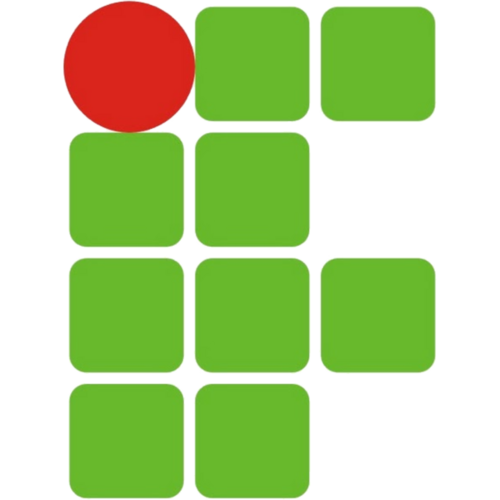
\includegraphics[scale=0.25]{IFRN}
		\end{flushleft}
	\end{minipage}		
	\begin{minipage}[c][1.5cm][c]{10.8cm}
		\begin{center}
			\resizebox{!}{0.3cm}{\textbf{Educação em Tecnologias Digitais}}\par
			\resizebox{!}{0.2cm}{\textbf{Instituto Federal de Educação, Ciência e Tecnologia do Rio Grande do Norte}}\par
			\resizebox{!}{0.2cm}{\today}
		\end{center}
	\end{minipage}
	
	\begin{center}
		Exercícios
	\end{center}
	
	\section{Sistemas Operacionais}
	
	\begin{enumerate}
		\item O que é sistema operacional?
		\item Cite algumas funções dos sistemas operacionais.
		\item Cite alguns dispositivos que utilizam sistemas operacionais.
		\item Quais são os sistemas operacionais mais conhecidos?
		\item Faça uma pesquisa breve sobre as versões do windows, desdo do lançamento até o presente.
		\item Pesquise algumas distribuições de linux disponíveis no mercado. 
		\item Qual o sistema operacional mais usando no mundo para computador e dispositivos móveis?
		\item Crie três área de trabalho no computador. Para cada uma delas, acesse o menu iniciar e abra um programa para cada área de trabalho: calculadora, explorador de arquivos e navegador web.
		\item Crie um atalho fixado na barra de tarefas para calculadora.
		\item Baixe os slides de aula, localize-o na pasta de download no explorador de arquivos. Na sequência envie o arquivo baixado para a lixeira. Confirme no explorador de arquivos se o arquivo baixado foi excluído. Depois, acesse a lixeira na área de trabalho e restaure o arquivo excluído. Por fim, acesso mais uma vez o explorador de arquivos e confirme se o arquivo deletado foi restaurado.
		\item Abra o programa bloco de notas no menu de arquivos. Maximize a janela do bloco de notas. Digite as informações textuais: nome completo, matrícula e nome do curso. Depois acesse o menu arquivo e escolha a opção salvar. Salve a nota no diretório documentos do seu computador com o nome "meus dados". Depois minimize a janela do seu bloco de notas. Na sequência acesse o explorador de arquivos e verifique se a nota foi salva em documentos. Acesse o bloco de notas minimizado na barra de tarefas, e por fim, feche a janela.
		\item Abra o explorador de arquivos. Acesse a pasta documentos. Crie uma nova pasta com o nome do seu curso. E dentro da pasta criada, crie subpastas para cada disciplina que você esteja cursando.
		\item Em configurações do sistema, escolha do modo de cores do seu windows para escuro.
		\item Coloque o seu computador no modo suspender. Espere alguns minutos. Em seguida, retorne ao sistema.
		\item Baixe os arquivos dos slides de aula, lista de exercícios e planejamento disciplina. Depois acesso o explorador de arquivos na opção downloads. Selecione todos os arquivos baixados e gere uma pasta compactada. E por fim, extraia a pasta compactada na área de trabalho do seu computador.
		\item Pesquise quais são os antivírus gratuitos disponível no mercado.
		\item Pesquise alguns tipos de vírus.
		\item O que é um backup?
		\item O que faz e qual a finalidade do desfragmentador de arquivos. 
	\end{enumerate}
	
	\section{Internet}
	
	\begin{enumerate}
		\item O que é internet?
		\item O que é uma URL, e em quantas partes é dividida?
		\item Cite alguns navegadores disponíveis no mercado, e quais suas vantagens.
		\item Acesse o navegador da sua preferência, e abra em abas separadas a página do IFRN e do SUAP.
		\item Salve a senha do SUAP no seu navegador.
		\item Marque a página do IFRN na lista de favoritos.
		\item Em uma janela anônima, acesse Outlook com sua conta do acadêmico.
		\item Em quantas parte é dividade um e-mail, e quais são elas?
		\item Envie uma mensagem via e-mail para um colega da sua turma. Na mensagem deve conter assunto, o texto redigido e uma cópia desta lista de exercício anexa.
		\item Envie uma mensagem via e-mail para um colega da sua turma, com cópia para um outro aluno. Na mensagem deve conter assunto, o texto redigido e uma cópia desta lista, os slides de aula em um único arquivo compactado.
		\item Acesse sua conta do OneDrive institucional, crie uma pasta com o nome da disciplina, e em seguida, inclua os slidades de aula e a lista de exercícios. Compartilhe a pasta que você criou com outro colega da sua turma.
		\item Crie um documento de texto no OneDrive, em seguida compartilhe com um colega, e por fim, escrevam no arquivo ao mesmo tempo.
	\end{enumerate}

\section{Ambiente Virtual de Aprendizagem}

	\begin{enumerate}
		\item Pesquise na internet ambientes virtual de aprendizagem disponíveis.
		\item Crie um documento com o Google Documentos diretamente na atividade criada no Google Sala de Aula. No corpo do documento aberto, digite o que motivou você a fazer o curso do IFRN. Feche a aba do documento no seu navegador. Em seguida, anexe uma cópia desta lista de exercício. E por fim, entregue a atividade.
	\end{enumerate}

\section{Segurança da Informação}

	\begin{enumerate}
		\item O que são os tipos de ameaças à segurança da informação (malware, phishing, ataque DDoS e Engenharia Social)? Dê exemplos.
		\item Cite algumas boas práticas para garantir à segurança da informação?
		\item Quais os direitos que a LGPD garante aos titulares dos dados?
	\end{enumerate}

\section{Inteligência Artificial na Educação}

	\begin{enumerate}
		\item Desafie o ChatGPT, Microsoft Copilot e Google Gemini a compor poesias de cordel sobre um determinado tema, em seguida compare cada poesia gerada.
		\item Utilize o Microsoft Copilot para gerar slogans, títulos e descrições criativas para produtos ou serviços.
		\item Utilize o Microsoft Copilot para gerar diferentes descrições para a mesma imagem, explorando sua criatividade e diferentes perspectivas.
		\item Utilize o Microsoft Copilot para gerar um resumo de um conteúdo de uma disciplina que você está cursando.
		\item Utilize o Microsoft Copilot para gerar uma lista de exercício com resposta de uma disciplina que você está cursando.
	\end{enumerate}

\end{document}